\chapter{Testes}
Três baterias de testes foram conduzidas ao longo da produção deste trabalho de graduação a fim de ver na prática o
impacto dos algoritmos de aprendizado de máquina quando aplicados em bases de dados com informações de rede.
Em um dos testes, a base utilizada foi a supracitada KDD Cup 99. Para os outros, utilizou-se uma série de dados
 gerados pelo mestrando da PUC-PR Eduardo Viegas, orientado pelo Prof. Dr. Altair Santin. Em ambos os casos, os algoritmos foram
 executados através do Weka.

\section{Weka}
O \textit{Waikato Environment for Knowledge Analysis} (Weka) é uma suíte de aplicações para aprendizagem de máquina e
mineração de dados. O software foi desenvolvido em Java na \textit{University of Waikato} e lincenciado sob a
\textit{GNU General Public License}. Os destaques dessa ferramenta incluem a vasta quantidade de algoritmos
implementados, pré-processamento de dados, seleção de atributos e visualização de dados. O Weka funciona como uma
interface, permitindo que novos algoritmos em Java sejam produzidos e facilmente executados de forma gráfica e com
resultados interativos \cite{bouckaert10}.

\section{Avaliação de Performance}
Gráficos ROC (\textit{Receiver Operating Characterístics}) são comumente usados como um método  para visualizar
a performance de classificadores e analisar as taxas de acertos e alarmes falsos \cite{fawcett04}. Um gráfico ROC
baseia-se em apenas duas classes: positivo ou negativo. Em termos de detecção de intrusão, uma conexão pode ser
considerada inofensiva (positivo) ou prejudicial (negativa). Para avaliar a precisão de um classificador,
duas outras categorias podem ser usadas: verdadeiro e falso. Quando cruzadas, obtém-se quatro possíveis resultados,
como mostra a tabela \ref{tab:tfpn}.

\begin{table}[h]
    \centering
    \caption{Categorias para análise de corretude}
    \label{tab:tfpn}
    \begin{tabular}{l|l|l|}
        \cline{2-3}
                                                               & \cellcolor[HTML]{EFEFEF}Verdadeiro (T)                                                           & \cellcolor[HTML]{EFEFEF}Falso (F)                                                     \\ \hline
        \multicolumn{1}{|l|}{\cellcolor[HTML]{EFEFEF}Positivo} & \begin{tabular}[c]{@{}l@{}}TP -- Conexão inofensiva é \\ classificada corretamente\end{tabular}  & \begin{tabular}[c]{@{}l@{}}FP -- Conexão anômala é \\ considerada normal\end{tabular} \\ \hline
        \multicolumn{1}{|l|}{\cellcolor[HTML]{EFEFEF}Negativo} & \begin{tabular}[c]{@{}l@{}}TN -- Conexão prejudicial é \\ classificada corretamente\end{tabular} & \begin{tabular}[c]{@{}l@{}}FN -- Conexão normal é \\ considerada anômala\end{tabular} \\ \hline
    \end{tabular}
\end{table}

Quando se sabe a verdadeira natureza dos casos de teste, é possível determinar a precisão, a taxa de Verdadeiro Positivo
 ($TP_{rate}$) e taxa de Falso Positivo ($FP_{rate}$). É possível inferir que uma das maiores preocupações ao se construir
 um A-NIDS é a minimização a taxa de Falso Positivo. Teoricamente se 100\% das conexões forem consideradas anômalas
 e bloqueadas, teremos $FP_{rate}$ igual a 0. Por um lado, o sistema estaria bloqueando conexões inofensivas, por outro,
 estaria com certeza evitando conexões ameaçadores. O cálculo das taxas se dá da seguinte maneira.

 $$ Precis\tilde{a}o = \frac{TP + TN}{P + N} $$
 $$ TP_{rate} = \frac{TP}{P} $$
 $$ FP_{rate} = \frac{FP}{N} $$

Essas taxas estão contidas no espaço entre $0$ e $1$, inclusivo, e são utilizadas para plotar o ROC. A $TP_{rate}$ é
usada no eixo $y$ e a $FP_{rate}$, no eixo $x$. Portanto, o gráfico ROC elicita a relação entre Verdadeiro Positivo e
Falso Positivo.
\par A Figura \ref{fig:roc} mostra uma curva ROC simples com 5 classificadores fictícios: A, B, C, D e E. Cada classificador
retorna um único ponto no espaço ROC. Se o ponto estiver localizado na coordenada (0,0), como o classificador A na
Figura \ref{fig:roc}, significa que nenhum caso foi considerado inofensivo. Classificadores que se encontram próximos ao eixo
$y$ podem ser considerados "conservadores", uma vez que necessitam de forte evidência para categorizar uma ocorrência
como positiva. Em contrapartida, o ponto B, posicionado em (1,1), representa sistemas que não acusariam nenhuma
conexão como anômala. Classificadores mais à direita do gráfico podem ser considerados "liberais" pois presumem como
positivo mais facilmente.

\begin{figure}
  \centering
    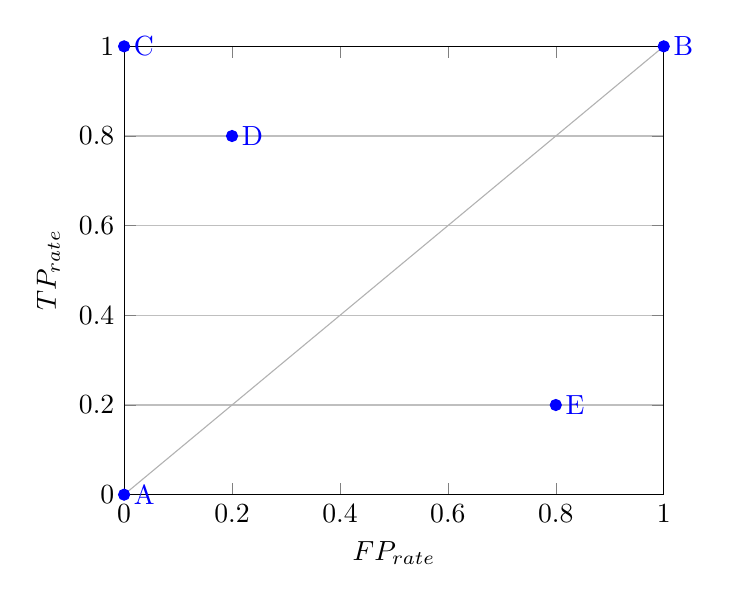
\begin{tikzpicture}
        \begin{axis}[
            xlabel={$FP_{rate}$},
            ylabel={$TP_{rate}$},
            xmin=0, xmax=1,
            ymin=0, ymax=1,
            ymajorgrids=true,
        ]
            \addplot[
                color=black!30,
                ]
                coordinates {
                (0,0)(1,1)
                };

            \addplot [ color=blue, mark=*, nodes near coords=A, every node near coord/.style={anchor=180}]
                coordinates {( 0, 0)};
            \addplot [ color=blue, mark=*, nodes near coords=B, every node near coord/.style={anchor=180}]
                coordinates {( 1, 1)};
            \addplot [ color=blue, mark=*, nodes near coords=C, every node near coord/.style={anchor=180}]
                coordinates {( 0, 1)};
            \addplot [ color=blue, mark=*, nodes near coords=D, every node near coord/.style={anchor=180}]
                coordinates {( 0.2, 0.8)};
            \addplot [ color=blue, mark=*, nodes near coords=E, every node near coord/.style={anchor=180}]
                coordinates {( 0.8, 0.2)};

        \end{axis}
    \end{tikzpicture}
    \caption{Exemplo da distribuição de 5 classificadores}
    \label{fig:roc}
\end{figure}

\par Um classificador perfeito resultaria no ponto (0,1), onde C se encontra. Isso significaria possuir $FP_{rate}$ de
0\% e $TP_{rate}$ de 100\%, ou seja, todas as conexões intrusivas serem detectadas e nenhuma conexão normal ser
bloqueada pelo sistema. Assim sendo, quanto maior o $TP_{rate}$ e menor o $FP_{rate}$, mais preciso é o algoritmo.
 Se um classificador está localizado abaixo da linha diagonal ($y = x$), isto significa que sua performance é pior do
 que a escolha aleatória de classes. O triângulo inferior direito é geralmente encontrado vazio pois em casos de
 classificação binária com alta taxa de erro, é possível simplesmente inverter os resultados. Portanto, E (0.8,0.2)
 seria tão preciso quanto D(0.2,0.8)


\section{Impacto de modelos representativos}
O primeiro teste realizado levou em consideração apenas o SVM padrão fornecido pelo libSVM para o Weka. A finalidade
era verificar o impacto da representabilidade da base de treino \cite{yaman11}, analisando a performance do algoritmo
quando treinado com bases de diferentes tamanhos. Para esse estudo, o KDD Cup 99 foi divido em 5 particionamentos,
cada um com tamanhos distintos de bases de treino e de testes, usando a opção de \textit{cross-validation} do Weka.
O comando executado incluiu um pré-processamento de heurística de encolhimento, peso $1$, \emph{seed} de $3$, erro de
$0.001$ e função núcleo \textit{Radial Basis}.

\begin{table}[h]
    \centering
    \caption{Comparação entre particionamentos de tamanhos diferentes}
    \label{tab:partic}
    \begin{tabular}{l|l|l|l|l|}
        \cline{2-5}
                                                        & \multicolumn{1}{c|}{\cellcolor[HTML]{EFEFEF}Tamanho Treino} & \multicolumn{1}{c|}{\cellcolor[HTML]{EFEFEF}Tamanho Teste} & \multicolumn{1}{c|}{\cellcolor[HTML]{EFEFEF}Tempo} & \multicolumn{1}{c|}{\cellcolor[HTML]{EFEFEF}Precisão} \\ \hline
        \multicolumn{1}{|l|}{\cellcolor[HTML]{EFEFEF}1} & 10\%                                                        & 90\%                                                       & 16h13m                                             & 92.22\%                                               \\ \hline
        \multicolumn{1}{|l|}{\cellcolor[HTML]{EFEFEF}2} & 20\%                                                        & 80\%                                                       & 24h02m                                             & 94.54\%                                               \\ \hline
        \multicolumn{1}{|l|}{\cellcolor[HTML]{EFEFEF}3} & 30\%                                                        & 70\%                                                       & 27h32m                                             & 95.65\%                                               \\ \hline
        \multicolumn{1}{|l|}{\cellcolor[HTML]{EFEFEF}4} & 40\%                                                        & 60\%                                                       & 32h11m                                             & 98.62\%                                               \\ \hline
        \multicolumn{1}{|l|}{\cellcolor[HTML]{EFEFEF}5} & 50\%                                                        & 50\%                                                       & 38h45m                                             & 99.64\%                                               \\ \hline
    \end{tabular}
\end{table}

\par A \ref{tab:partic} mostra os as proporções de base de testes e treino em cada particionamento e seus respectivos
resultados. É possível notar uma clara correlação entre o tamanho da base de treino e a porcentagem de acertos. O
melhor resultado foi de $99.64$\% quando metade da base foi usada para gerar o modelo. Entretanto, em uma situação real
não há dados disponíveis o suficiente para se representar metade das transmissões que ocorrem diariamente.


\section{Impacto da imprevisibilidade}
Uma abordagem recente direcionou os estudos desse trabalho para a análise da real capacidade de algoritmos de
aprendizado de máquinas em se adaptar a novas realidades e detectar ameaças totalmente desconhecidas \cite{sommer10}.
\par Através de simulações de rede, foi gerado um conjunto de dados, contendo conexões normais e anômalas,
dispostos em três grupos distintos, os quais chamaremos de \textit{Inicial}, \textit{Análogo} e \textit{Desconhecido}.
O primeiro é um limitado conjunto de conexões utilizando protocolos HTTP e SMTP. Este foi dividido em dois grupos:
um para treino, com $258880$ instâncias, e outro para testes, com $275204$. O grupo \textit{Análogo} possui dados de
$148343$ conexões e, como o nome sugere, possui ataques semelhantes ou derivados daqueles no grupo anterior.
Já o terceiro engloba, também, ataques completamente desconhecidos provenientes de outros
protocolos, como SNMP e SSH, totalizando $276548$ ocorrências. Apenas o grupo \textit{Inicial} foi utilizado para
treino. O objetivo é observar o comportamento do sistema quando novos
ataques são recebidos, sejam eles derivados dos conhecidos ou completamente novos.
\par Tanto o SVM quanto DT foram utilizados nesta análise. As tabelas \ref{tab:dt} e \ref{tab:svm} mostram os resultados
em cada etapa do processo, em termos de taxa de Verdadeiro Positivo, taxa de Falso Positivo, tempo para classificar
todas as instâncias da respectiva base, precisão e porcentagem de instâncias classificadas corretamente. As taxas de
acerto evidenciam uma grande perda de confiabilidade conforme o surgimento de novos ataques, sendo a classificação da
base \textit{Desconhecido} praticamente tão eficiente quanto uma adivinhação aleatória.

\begin{table}[h]
    \centering
    \caption{Resultados de DT em cada base}
    \label{tab:dt}
    \begin{tabular}{l|l|l|l|l|l|}
        \cline{2-6}
                                                                   & \multicolumn{5}{c|}{\cellcolor[HTML]{EFEFEF}DT}        \\ \cline{2-6}
                                                                   & $TP_{rate}$ & $FP_{rate}$ & Tempo & Acertos & Precisão \\ \hline
        \multicolumn{1}{|l|}{\cellcolor[HTML]{EFEFEF}Inicial}      & 0.982       & 0.018       & 6.92s & 98.18\% & 0.982    \\ \hline
        \multicolumn{1}{|l|}{\cellcolor[HTML]{EFEFEF}Análogo}      & 0.912       & 0.856       & 3.73s  & 91.23\% & 0.885    \\ \hline
        \multicolumn{1}{|l|}{\cellcolor[HTML]{EFEFEF}Desconhecido} & 0.503       & 0.497       & 6.95s & 50.29\% & 0.751    \\ \hline
    \end{tabular}
\end{table}

\begin{table}[h]
    \centering
    \caption{Resultados de SVM em cada base}
    \label{tab:svm}
    \begin{tabular}{l|l|l|l|l|l|}
        \cline{2-6}
                                                                   & \multicolumn{5}{c|}{\cellcolor[HTML]{C0C0C0}SVM}          \\ \cline{2-6}
                                                                   & $TP_{rate}$ & $FP_{rate}$ & Tempo    & Acertos & Precisão \\ \hline
        \multicolumn{1}{|l|}{\cellcolor[HTML]{EFEFEF}Inicial}      & 0.971       & 0.029       & 15h13min & 98.43\%  & 0.984     \\ \hline
        \multicolumn{1}{|l|}{\cellcolor[HTML]{EFEFEF}Análogo}      & 0.902       & 0.845       & 8h12min  & 90.27\%  & 0.891    \\ \hline
        \multicolumn{1}{|l|}{\cellcolor[HTML]{EFEFEF}Desconhecido} & 0.52        & 0.484       & 15h29min & 50.78\%  & 0.753     \\ \hline
    \end{tabular}
\end{table}



\section{Impacto da seleção de atributos}
Tendo em vista o alto custo computacional para processar as 51 características iniciais, foi ponderada a viabilidade
de se utilizar uma seleção de atributos prévia para agilizar o processamento na tomada de decisões. Utilizando o
PCA, a quantidade de características foi reduzida para 39. Novos testes foram executados, seguindo o mesmo método da
análise anterior.

\begin{table}[h]
    \centering
    \caption{Resultados de DT em cada base com seleção de atributos}
    \label{tab:dtattrless}
    \begin{tabular}{l|l|l|l|l|l|}
        \cline{2-6}
                                                                   & \multicolumn{5}{c|}{\cellcolor[HTML]{EFEFEF}DT}        \\ \cline{2-6}
                                                                   & $TP_{rate}$ & $FP_{rate}$ & Tempo & Acertos & Precisão \\ \hline
        \multicolumn{1}{|l|}{\cellcolor[HTML]{EFEFEF}Inicial}      & 1.0         & 0.0         & 5.75s & 99.98\% & 1.0      \\ \hline
        \multicolumn{1}{|l|}{\cellcolor[HTML]{EFEFEF}Análogo}      & 0.848       & 0.429       & 3.1s  & 84.82\% & 0.914    \\ \hline
        \multicolumn{1}{|l|}{\cellcolor[HTML]{EFEFEF}Desconhecido} & 0.499       & 0.501       & 5.78s & 49.86\% & 0.414    \\ \hline
    \end{tabular}
\end{table}

\begin{table}[h]
    \centering
    \caption{Resultados de SVM em cada base com seleção de atributos}
    \label{tab:svmattrless}
    \begin{tabular}{l|l|l|l|l|l|}
        \cline{2-6}
                                                                   & \multicolumn{5}{c|}{\cellcolor[HTML]{C0C0C0}SVM}          \\ \cline{2-6}
                                                                   & $TP_{rate}$ & $FP_{rate}$ & Tempo    & Acertos & Precisão \\ \hline
        \multicolumn{1}{|l|}{\cellcolor[HTML]{EFEFEF}Inicial}      & 0.503       & 0.502       & 14h45min & 50.3\%  & 0.75     \\ \hline
        \multicolumn{1}{|l|}{\cellcolor[HTML]{EFEFEF}Análogo}      & 0.068       & 0.068       & 7h56min  & 6.78\%  & 0.937    \\ \hline
        \multicolumn{1}{|l|}{\cellcolor[HTML]{EFEFEF}Desconhecido} & 0.5         & 0.5         & 14h51min & 50.0\%  & 0.75     \\ \hline
    \end{tabular}
\end{table}

As tabelas \ref{tab:dtattrless} e \ref{tab:svmattrless} mostram que o resultado dos algoritmos nesse
cenário teve nenhum ganho significativo. Enquanto os atributos selecionados podem ser mais descritivos para os
ataques vistos na base \textit{Inicial}, talvez não sejam interessantes para identificar os ataques que residem além
daquele horizonte.
 A figura \ref{fig:roctest} evidencia uma diminuição de Falso Positivo na base \emph{Análogo}
 quando usada a seleção de atributo, mas ainda sendo muito superior ao \textit{Inicial}. O comportamento
 ao se classificar a base totalmente desconhecida mostrou-se tão bom quanto escolha aleatória.

\begin{figure}[h]
  \centering
    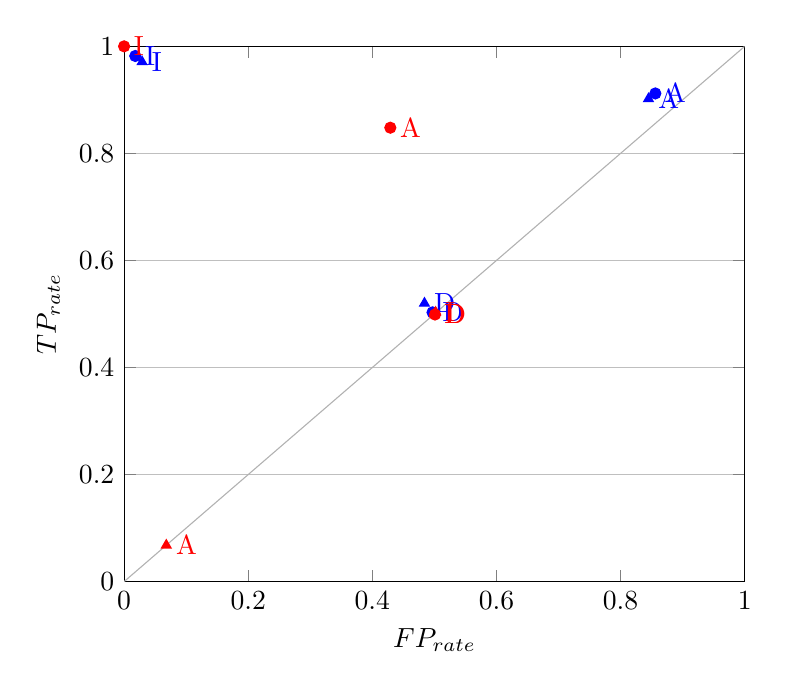
\begin{tikzpicture}
        \begin{axis}[
        scale only axis,
        width=0.65\textwidth,
            xlabel={$FP_{rate}$},
            ylabel={$TP_{rate}$},
            xmin=0, xmax=1,
            ymin=0, ymax=1,
            ymajorgrids=true,
        ]
            \addplot[
                color=black!30,
                ]
                coordinates {
                (0,0)(1,1)
                };

            %  DT
            \addplot [ color=blue, mark=*, nodes near coords=I, every node near coord/.style={anchor=180}]
                coordinates {( 0.018, 0.982)};
            \addplot [ color=blue, mark=*, nodes near coords=A, every node near coord/.style={anchor=180}]
                coordinates {( 0.856, 0.912 )};
            \addplot [ color=blue, mark=*, nodes near coords=D, every node near coord/.style={anchor=180}]
                coordinates {( 0.497, 0.503 )};

            %  SVM
            \addplot [ color=blue, mark=triangle*, nodes near coords=I, every node near coord/.style={anchor=180}]
                coordinates {( 0.029, 0.971)};
            \addplot [ color=blue, mark=triangle*, nodes near coords=A, every node near coord/.style={anchor=180}]
                coordinates {( 0.845, 0.902)};
            \addplot [ color=blue, mark=triangle*, nodes near coords=D, every node near coord/.style={anchor=180}]
                coordinates {( 0.484, 0.52)};

            %  DT_attrless
            \addplot [ color=red, mark=*, nodes near coords=I, every node near coord/.style={anchor=180}]
                coordinates {( 0, 1)};
            \addplot [ color=red, mark=*, nodes near coords=A, every node near coord/.style={anchor=180}]
                coordinates {( 0.429, 0.848)};
            \addplot [ color=red, mark=*, nodes near coords=D, every node near coord/.style={anchor=180}]
                coordinates {( 0.501, 0.499)};

            %  SVM
            \addplot [ color=red, mark=triangle*, nodes near coords=I, every node near coord/.style={anchor=180}]
                coordinates {( 0.502, 0.503)};
            \addplot [ color=red, mark=triangle*, nodes near coords=A, every node near coord/.style={anchor=180}]
                coordinates {( 0.068, 0.068)};
            \addplot [ color=red, mark=triangle*, nodes near coords=D, every node near coord/.style={anchor=180}]
                coordinates {( 0.5, 0.5)};

        \end{axis}
    \end{tikzpicture}
    \caption{Comparativo dos algoritmos SVM (triângulo) e DT (círculo) em base sem e com seleção de
    atributo (azul e vermelho, respectivamente). I -- \textit{Inicial};  A -- \textit{Análogo};
     D -- \textit{Desconhecido}}
    \label{fig:roctest}
\end{figure}